%===================================================================================================
%  Chapter : 真空中の電磁波
%  説明    : マクスウェル方程式をもとに,真空中の電磁波の波動方程式を導出し,
%            また,電磁波の性質について考える
%===================================================================================================
%   %==========================================================================
%   %  SubSection
%   %==========================================================================
    \section{波動方程式}
        \begin{mycomment}
            最初に,波動方程式について,簡単にまとめておこう
            \footnote{
                詳細は,微分方程式の教科書を参照すること.
            }.
        \end{mycomment}

    \subsection{波動関数}
        波動方程式の解は \textbf{波動関数} である.波動関数とは,実際の現象として
        起きている \textbf{波} もしくは \textbf{波動} を,数学的な関数として抽象化
        したものである.これにより,波という現象を数学的に解析できるようになる.
        波動方程式を考える前に,\textbf{波} もしくは \textbf{波動} について調べておく
        必要がある.


    \subsection{波動方程式の導出}
        2つの独立変数 $x$,$t$ をもつ関数 $K(x,\,t)$ に関する \textbf{波動方程式} とは,
        以下の偏微分方程式のことを言う.
        \begin{align}
            \frac{{\rd}^{2} K}{{\rd t}^{2}}  = a \frac{{\rd}^{2}K}{{\rd x}}.
        \end{align}

%   %==========================================================================
%   %  Section
%   %==========================================================================
    \section{真空中のマクスウェル方程式}
        \begin{mycomment}
        前章で確認した 微分形のマクスウェル方程式 を用いて,電磁波について考える.
        まず,電場の波動方程式 と 磁束密度の波動方程式 を
        別々に確認する.そして,ファラデーの電磁誘導の法則 と 電場に対する
        ガウスの法則から,それら2つの波動方程式の関係を考える.
        \end{mycomment}

%   %==========================================================================
%   %  SubSection
%   %==========================================================================
    \subsection{マクスウェル方程式の確認}
        マクスウェルの方程式を書き下しておく.
        \begin{align}
            \drot \bE
            &=
            -\frac{\rd \bB}{\rd t}\\
            \drot\bB
            &=
            \mu_{0}\left(\bi+
                \varepsilon_{0}\frac{\rd \bE}{\rd t}
            \right)\\
            \ddiv\bE
            &=\frac{\rho}{\varepsilon_{0}}\\
            \ddiv\bB
            &=
            0\\
        \end{align}

%   %==========================================================================
%   %  SubSection
%   %==========================================================================
    \subsection{真空中であることの仮定}
        電磁波を考えるにあたって 話を簡単にするために,以下の仮定を設ける.これは
        真空中の電磁波を考えることによる要請である.
        \begin{enumerate}
        \item 電荷密度 $\rho$ の分布はないものとする.
                                \begin{align}
                                \rho
                                =0
                                \end{align}
        \item 電流密度 $\bi$ の分布はないものとする.
                                \begin{align}
                                \bi
                                =0
                                \end{align}
        \end{enumerate}




%   %==========================================================================
%   %  SubSection
%   %==========================================================================
    \subsection{電場の波動方程式}
            ファラデーの電磁誘導
            の法則 $\drot \bE=-\rd \bB/\rd t$ の
            両辺に $\drot$ をとる.
                                    \begin{align}
                                    \mathrm{rot\,rot} \bE
                                    &=
                                    -\drot\frac{\rd \bB}{\rd t}
                                    \end{align}
            ここで,ベクトル解析の公式 $\mathrm{rot\, rot}=\mathrm{grad\, div}-\Delta$ を適用する
                \footnote{
                    ここに,
                        \begin{align*}
                            \Delta:=
                            \mathrm{div\, grad}=
                            \frac{\rd^{2}}{\rd x^{2}}+
                            \frac{\rd^{2}}{\rd y^{2}}+
                            \frac{\rd^{2}}{\rd z^{2}}
                        \end{align*}
                    である.
                }.
            すると,
            \begin{align}\label{denjiha1}
                \mathrm{grad\, div}\,\bE-\Delta\,\bE
                &=
                -\drot\frac{\rd \bB}{\rd t}
            \end{align}
            となる.この式の右辺第1項の $\mathrm{grad\, div}\,\bE$ に注目する.
            電場に対するガウスの法則は,仮定の $\rho=0$ によって,
            \begin{align*}
                \ddiv\bE
                =\frac{1}{\varepsilon_{0}}\rho
                =0
            \end{align*}
            である.従って,$\dgrad0=0$ となって,式(\ref{denjiha1})は
            \begin{align}
                \Delta\,\bE
                &=
                \drot\frac{\rd \bB}{\rd t}
            \end{align}
            と計算される.回転 $\drot$ と時間微分 $\rd/\rd t$ は可換であるから
            \begin{align}\label{denjiha2}
                \Delta\,\bE
                &=
                \frac{\rd (\drot\bB)}{\rd t}
            \end{align}

            ところで,左辺の $\drot\bB$ は アンペール$=$マクスウェルの法則 から
            \begin{align*}
                \drot\bB = \mu_{0}\varepsilon_{0}
                \frac{\rd \bE}{\rd t}
            \end{align*}
            である.ここで,仮定により $\bi=0$ を考慮した.
            これを,式(\ref{denjiha2})に代入して,
            \begin{align}
                \Delta\,\bE &=
                \frac{\rd }{\rd t}\left(\mu_{0}\varepsilon_{0}
                \frac{\rd \bE}{\rd t}\right)\notag \\
                \Leftrightarrow
                \Delta\,\bE
                &=
                \mu_{0}\varepsilon_{0}
                \frac{\rd^{2} \bE}{\rd t^{2}}
            \end{align}
            である.この式を以下のように変形する.
            \begin{align}\label{denjiha3}
                \left(\Delta-\mu_{0}\varepsilon_{0}
                \frac{\rd^{2}}{\rd t^{2}}\right)\bE
                &=0
            \end{align}
            この式は波動方程式と同型である.従って,電場は波動として伝わることを意味する.

            電場の波の位相速度を考える.
            そのために,速度 $\bv$ の位相速度をもつ波動の方程式 $\textit{\textbf{K}}(\br,t)$ を
            書き下す.
            \begin{align}\label{denjiha4}
                \left(\Delta-\frac{1}{v^{2}}
                \frac{\rd^{2}}{\rd t^{2}}\right)\textit{\textbf{K}}
                &=0
            \end{align}
            この式(\ref{denjiha3})と式(\ref{denjiha4})とを見比べてみると,電場の波動方程式の位相速度は
            \begin{align}
                \frac{1}{v^{2}}=\mu_{0}\varepsilon_{0} \notag \\
                \Leftrightarrow
                v=\frac{1}{\sqrt{\mu_{0}\varepsilon_{0}}}
            \end{align}
            である.

            速度を具体的に計算してみるよう.まず,以下の定数は既知である.
            \begin{align*}
                \varepsilon_{0} &= \frac{1}{36\pi\times 10^{9}}\, \mathrm{[F/m]}, \\
                \mu_{0}         &= \frac{4\pi}{ 10^{7}}\, \mathrm{[H/m]}.
            \end{align*}
            これを先の位相速度の式に代入して計算すると,
            \begin{align}
                \frac{1}{\sqrt{\mu_{0}\varepsilon_{0}}}
                &= \frac{1}{\sqrt{\frac{1}{36\pi\times 10^{9}}\,\mathrm{[F/m]} \cdot \frac{4\pi}{ 10^{7}}\,\mathrm{[H/m]}}} \notag \\
                &= 3\times 10^{8} \mathrm{[m/s]}
            \end{align}
            となって,これは光速にかなり近い値である

            この値の妥当性は,ヘルツらの実験により,光速と同等であることが確認された.
            そこで,改めて光速を $c$ と表すことにする
                \footnote{
                    実際は,光速を実験的に測定し,その値に基づいて,$\varepsilon_{0}$ の値が決められている.
                    $\mu_{0}=4\pi \times 10^{-7}$ と定義されているので(電流の定義の項目を参照),
                    光速 $c$ を測り, $c=1/\sqrt{\varepsilon_{0} \mu_{0}}$ の関係から $\varepsilon_{0}$ を計算できる.
                }.
            \begin{align}
                c:=\frac{1}{\sqrt{\varepsilon_{0}\mu_{0}}}\cong 3\times 10^{8} \,\, \mathrm{[m/s]}
            \end{align}

            光速 $c=1/\sqrt{\varepsilon_{0} \mu_{0}}$ を用いて,電場 $\bE$ の波動方程式を表せば,
            \begin{align}
                \left(\Delta-\frac{1}{c^{2}}
                \frac{\rd^{2}}{\rd t^{2}}\right)\bE
                &=0
            \end{align}
            である.

             先ほどは次元の具体的な計算をして指定なかった.次元が速度になることをここで確かめておこう.
             確かめたい次元は
                \[
                    \frac{1}{\sqrt{\mathrm{[F/m]} \mathrm{[H/m]}}} = \mathrm{[m/s]}
                \]
            となることである.次元の括弧を書くのは面倒なので,この計算では省略して記述する.
            まずは,以下のようになることは,簡単にわかる.
                \[
                    \frac{1}{\sqrt{\mathrm{(F/m)} \cdot \mathrm{(H/m)}}} = \frac{1}{\sqrt{\mathrm{FH}/\mathrm{m}^{2}}}.
                \]
            次に $\mathrm{FH}$ の計算を行いたいが,おそらく単位の定義も忘れているだろうから,定義に戻って計算しよう.
            [F]は静電容量の単位で,単位電圧1[V]あたりにためることのできる電荷量[C]$=$[A$\cdot$s]で定義される.
                \[
                    \mathrm{F} := \frac{\mathrm{A}\cdot\mathrm{s}}{\mathrm{V}}.
                \]
            [H]はインダクタンスの単位で,単位時間1[s]の間に1[A]の電流が流れる場合に,
            1[V]の電圧が生じる回路のインダクタンスとして定義される.
                \[
                    \mathrm{H} := \frac{\mathrm{V}}{\mathrm{A/s}} = \frac{\mathrm{V}\cdot\mathrm{s}}{\mathrm{A}}.
                \]
            だから,
                \[
                    \mathrm{F}\cdot\mathrm{H} = \mathrm{s}^{2}.
                \]
            要するに,
                \[
                    \frac{1}{\sqrt{\mathrm{F/m} \mathrm{H/m}}}  = \frac{1}{\sqrt{\mathrm{s}^{2}/\mathrm{m}^{2}}}
                                                                = \frac{1}{\mathrm{s}/\mathrm{m}}
                                                                = \mathrm{m}/\mathrm{s}
                \]
            となり,次元が速度になることが確かめられた.

%   %==========================================================================
%   %  SubSection
%   %==========================================================================
    \subsection{磁束密度の波動方程式}
            今度は,磁束密度の波動方程式を考える.(導出方法は電場の波動方程式とほぼ同じである.)
            アンペール$=$マクスウェル
            の法則 $\drot\bB=\varepsilon_{0}\mu_{0}(\rd \bE/\rd t)$ の
            両辺に,回転 $\drot$ をとる.(仮定により,$\bi=0$ であることを考慮した.)
                \begin{align}
                    \mathrm{rot\,rot}\bB
                    =\varepsilon_{0}\mu_{0}\drot
                    \frac{\rd \bE}{\rd t}
                \end{align}
            そして,左辺に ベクトル解析の公式 $\mathrm{rot\, rot}=\mathrm{grad\, div}-\Delta$ を適用する.
                \begin{align}
                    \mathrm{grad\, div}\bB- \Delta \bB
                    =\varepsilon_{0}\mu_{0}\drot
                    \frac{\rd \bE}{\rd t}
                \end{align}
            ここで,磁束密度に対するガウスの法則$\ddiv\bB=0$ によって,
            第一項は 0 になる.
                \begin{align}
                    -\Delta \bB
                    =\varepsilon_{0}\mu_{0}\drot
                    \frac{\rd \bE}{\rd t}
                \end{align}
            回転 $\drot$ と時間微分 $\rd /\rd t$ は可換であるから
                \begin{align}
                    -\Delta \bB
                    =\varepsilon_{0}\mu_{0}
                    \frac{\rd (\drot\bE)}{\rd t}
                \end{align}
            とできる.ここで,
            ファラデーの電磁誘導より
            の法則 $\drot \bE
            =\rd \bB/\rd t$ であるから,
                \begin{align}
                    -\Delta \bB
                    &=-\varepsilon_{0}\mu_{0}
                    \frac{\rd }{\rd t}\left(\frac{\rd \bB}{\rd t}\right) \notag \\
                    \Leftrightarrow\quad
                    \Delta \bB
                    &=\varepsilon_{0}\mu_{0}
                    \frac{\rd^{2} \bB}{\rd t^{2}}
                \end{align}
            この式を整理すると,
                \begin{align}
                    \left(\Delta-\varepsilon_{0}\mu_{0}\frac{\rd^{2}}{\rd t^{2}}\right)\bB=0
                \end{align}
            である.光速 $c$ を用いると,
                                \begin{align}
                                    \left(\Delta-\frac{1}{c^{2}}
                                    \frac{\rd^{2}}{\rd t^{2}}\right)\bB
                                     &=0
                                     \end{align}
            である.
            この式は波動方程式と同型である.

            従って,磁束密度も光速 $c$ で伝播することがわかる.

%   %==========================================================================
%   %  SubSection
%   %==========================================================================
    \subsection{光速}
        この速度は,「どの慣性系」に対する物でもない.
        どんな慣性系でも全く同じ光速を観測し得る.これは特殊相対性理論の
        基本要請の一つであり,\textbf{光速度不変の原理} とよばれる.

        ある慣性系 O で光速 $c$ を観測したとする.また,その慣性系 O において,光速と同じ速度で
        運動する別の慣性系 O$'$ も観測したとする.ガリレイ変換を考えれば,
        慣性系 O$'$ で光速 $c'$ を測定すれば,$c'=0$ である.しかし,光速度不変の原理によれば,
        慣性系 O$'$ から光速を測定しても,その速度は $c=c'$ であるという
        (従って,光速度不変の原理を採用すると,ガリレイ変換は成り立たない.)

        この原理を説明する実験事実として多くの教科書では,\textbf{マイケルソンとモーレイの実験} 取り上げられている.
        ここら辺から「特殊相対性理論」の領域になる.今は電磁気学を考えているので,この辺でこの話を
        止めておく.

%   %==========================================================================
%   %  SubSection
%   %==========================================================================
    \subsection{電磁波の伝搬}
            上の計算によって,電場と磁束密度の波動方程式を得た.しかし,
            波には \textbf{縦波} と \textbf{横波} の2種類
            が存在する.
            ここでは,電場もしくは磁束密度は,縦波か横波かを
            考えていくことにしよう.

            先に電場の波動について考える.それには,微分形の電場に対するガウスの法則
            を用いる.仮定より,電荷密度は存在しないので,電場に対するガウスの法則は
            \begin{align}\label{den_hadou}
            \ddiv\bE=0
            \end{align}
            である.電場の波動方程式 $\displaystyle\left(\Delta-\frac{1}{{c}^{2}}
            \frac{\rd^{2}}{\rd t^{2}}\right)\bE=0$ を満たす解は
            \begin{align}\label{eq:denbaba}
            \bE=f\left(\br\cdot\textit{\textbf{k}}+ct\right)
            +g\left(\br\cdot\textit{\textbf{k}}-ct\right)
            \end{align}
            で表されるので
              \footnote{
                  本節末のメモを参照.
              }
            ,この式を式(\ref{den_hadou})に代入すると,
            \begin{align*}
                    \ddiv\{f\left(\br\cdot\textit{\textbf{k}}+ct\right)
                    +g\left(\br\cdot\textit{\textbf{k}}-ct\right)\}=0
            \end{align*}
                        $\ddiv$ を具体的に表示すると,
            \begin{align*}
                    \left(\frac{\rd }{\rd x}+\frac{\rd }{\rd y}+\frac{\rd }{\rd z}\right)\{ f+g \} =0
            \end{align*}
            ここで,式を見やすくするために,
                        \begin{align*}
                f&:=f\left(\br\cdot\textit{\textbf{k}}+ct\right) \,,\, \\
                g&:=g\left(\br\cdot\textit{\textbf{k}}-ct\right)
            \end{align*}
            と省略して
            書くことにした.微分作用素を展開して具体的に関数に作用させると,
            \begin{align*}
                0 = \frac{\rd }{\rd x}\{ f+g\} + \frac{\rd }{\rd y}\{ f+g\} + \frac{\rd }{\rd z}\{ f+g\}
            \end{align*}
            $f$,$g$ は電場の波動の進行方向 $\textbf{\textit{k}}$ を含むことに注意すれば
            \begin{align*}
                    0 &=k_{x}\biggl\{\frac{\rd f}{\rd x}+\frac{\rd g}{\rd x}\biggr\} \\
                      &\quad  + k_{y}\biggl\{\frac{\rd f}{\rd y}+\frac{\rd g}{\rd y}\biggr\} \\
                      &\qquad + k_{z}\biggl\{\frac{\rd f}{\rd z}+\frac{\rd g}{\rd z}\biggr\}
            \end{align*}
            となる.これは明らかに,以下のように内積の形
            で表現できることがわかる.
            \begin{align*}
            0&=(k_{x},\,k_{y},\,k_{z})\left(\, \frac{\rd f}{\rd x}+\frac{\rd g}{\rd x}\,\,,\,\,\,
            \frac{\rd f}{\rd y}+\frac{\rd g}{\rd y}\,\,,\,\,\,
            \frac{\rd f}{\rd z}+\frac{\rd g}{\rd z}\,
            \right)\notag \\
            &=(k_{x},\,k_{y},\,k_{z})\cdot\left(\, f_{x}'+g_{x}'\,\,,\,\,\,
            f_{y}'+g_{y}'\,\,,\,\,\,
            f_{z}'+g_{z}'\,\right)
            \notag \\
            &=\textbf{\textit{k}}\cdot(\textbf{\textit{f}}'+\textbf{\textit{g}}')
            \end{align*}
            ここで電場の式(\ref{eq:denbaba});
            \begin{align*}
                \bE=f\left(\br\cdot\textit{\textbf{k}}+vt\right) + g\left(\br\cdot\textit{\textbf{k}}-ct\right)
            \end{align*}
            を思い起こせば,
            \begin{align}
                \textbf{\textit{k}}\cdot\bE'=0
            \end{align}

            電場の空間微分 $\bE'$ は電場の変化の方向
            を表現していて, $\textbf{\textit{k}}$ は電場の波動の
            進行方向である.これら2つの内積が 0 であるという結果から,
            \textbf{電場は,進行方向と垂直な方向に,その振幅が変化する} ということがわかる.
            進行方向と垂直な方向に変化するということは,
            \textbf{電場の波動は横波である} ということを意味する.

            磁束密度についても同様に考えることができて,
            \begin{align}
            \textbf{\textit{k}}\cdot\bB'=0
            \end{align}
            の関係が得られる.つまり,\textbf{磁束密度の波動は横波である} ということもわかる.


        \begin{memo}{波動方程式}
          波動とその運動について考える.波動の運動を表す方程式のことを,\textbf{波動方程式} という.
          波動の形は,関数で表すことができ,これを \textbf{波動関数} という.

          図\ref{fig:wave_eq001}は,波動の進行方向を $z$,振動の方向を $x$,時間の経過を $t$ 軸で
          表現したものである.
                        \begin{figure}[hbt]
                            \begin{center}
                                \includegraphicslarge{wave_eq001.pdf}
                                \caption{波動の時間移動}
                                \label{fig:wave_eq001}
                            \end{center}
                        \end{figure}


          波動関数は,もとっとも単純な形をしている,$\sin$ 型や $\cos$ 型でかまわなのだが,
          より一般的な波動をイメージして現象を考えたいので,ここでは,任意の形をした
          波形を考える.この波の波動関数を $f$ とおこう.このとき,波動関数は,$f(z-vt)$ の形
          で表せる.その理由を,以下で説明する.

          図\ref{fig:wave_eq001}を参照してもらいたい.$x$,$z$,$t$ の交点(原点)を,
          時刻 $t=0$ とし,$t_{0}$ で表す.
          時刻 $t_{0}$ から時間 $\Delta t$ 後の時刻を $t_{1}$ とする.
          そして,時刻 $t_{0}$ での波動関数の位置は $z_{0}$ であるとし,
          時刻 $t_{1}$ での波動関数の位置は $z_{1}$ とする.
          波動の $z$ 軸の移動速度は $v_{z}$ であるとする.

          この時,
          時刻 $t_{0}$ の波動関数は $f_{0}:=f(z_{0}-v_{z}t_{0})$ と表せる
            \footnote{
                記号「$:=$」は,左辺を右辺により定義することを意味する.
            }.
          では,時刻 $t_{0}$ における波動関数はどうだろうか.
              \begin{equation*}
                  z_{0} = z_{1} - v_{z} \Delta t
              \end{equation*}
          であることに注意すると,$t_{1}$ は
              \begin{equation*}
                  t_{1} = t_{0} + \Delta t
                  \quad \Leftrightarrow \quad
                  \Delta t = t_{1} - t_{0}
              \end{equation*}
          と表せることから,
              \begin{align*}
                  z_{0} &= z_{1} - v_{z} \Delta t            \\
                        &= z_{1} - v_{z} ( t_{1} - t_{0} )   \\
                        &= z_{1} - v_{z}t_{1}  + v_{z}t_{0}  \\
                  \therefore\quad
                  z_{0} -  v_{z}t_{0} &=  z_{1} - v_{z}t_{1}.
              \end{align*}
          従って,$f(z_{1} -  v_{z}t_{1}) = f(z_{0} -  v_{z}t_{0})$ が成立する.
          以上により,波動関数は $f(z-vt)$ で表せることがわかった.
          よって,波動関数は時間経過でその形$f$を変えずに移動することがわかる.
          また同様に,$f(z+vt)$ の形であっても,時間経過による波形の変化はないことを
          示すことができる.
        \end{memo}



%   %==========================================================================
%   %  SubSection
%   %==========================================================================
    \subsection{電場と磁束密度の伝搬関係}
        次に,電場の波動 と 磁束密度の波動 の関係を調べていこう.
        それには,ファラデーの電磁誘導の法則を使う.
        再度式を書き下す.
                        \begin{align}
                            -\frac{\rd \bB}{\rd t}
                            &=\mathrm{rot\,} \bE
                        \end{align}
        この後の式変形のために,この式を成分表示で書き表しておく.
        \begin{align}\label{dennpann1}
        \left(
        \begin{array}{cc}
        -\displaystyle\frac{\rd B_{x}}{\rd t} \\
        -\displaystyle\frac{\rd B_{y}}{\rd t} \\
        -\displaystyle\frac{\rd B_{z}}{\rd t}
        \end{array}
        \right)
        =
        \left(
            \begin{array}{cc}
            \displaystyle\frac{\rd E_{z}}{\rd y}-\frac{\rd E_{y}}{\rd z}\\
            \displaystyle\frac{\rd E_{x}}{\rd z}-\frac{\rd E_{z}}{\rd x} \\
            \displaystyle\frac{\rd E_{y}}{\rd x}-\frac{\rd E_{x}}{\rd y}
            \end{array}
            \right)
        \end{align}

        電場が時間変化するとその周辺に磁束密度が発生する.
        逆に,磁束密度が時間変化するとその周辺には電場が発生する.
        ここでは,電場の伝搬を考えて,その電場の波動の変化に対して
        どのように磁束密度が生れ,どのように伝搬するかを
        考えていくことにする.
        ここで次のような仮定を設ける.すなわち,

        \begin{enumerate}
        \item 電場の伝搬方向は $z$ 軸正の向きとする.
        \item 電場の振幅変化の方向は $x$ 軸方向とする.
        \end{enumerate}
        上の2つの仮定から,
        電場は以下のように成分表示される.

        \begin{align}\label{dennpann2}
        \left(
        \begin{array}{cc}
        E_{x} \\
        E_{y} \\
        E_{z}
        \end{array}
        \right)
        =
        \left(
        \begin{array}{cc}
        f(z-ct) +g(z+ct)\\
        0 \\
        0
        \end{array}
        \right)
        \end{align}


        この仮定は先ほど得た結果,つまり,電場の波動と磁束密度の波動は
        横波であるということから,設定できる.

        電磁誘導の法則の式(\ref{dennpann1})に,電場の式(\ref{dennpann2})を
        代入し整理すれば,
        \begin{align*}
        &\left(
        \begin{array}{cc}
        -\displaystyle\frac{\rd B_{x}}{\rd t} \\
        -\displaystyle\frac{\rd B_{y}}{\rd t} \\
        -\displaystyle\frac{\rd B_{z}}{\rd t}
        \end{array}
        \right)  \notag \\
        &\quad =
        \left(
        \begin{array}{cc}
        \displaystyle\frac{\rd }{\rd y}0-\frac{\rd }{\rd z}0\\
        \displaystyle\frac{\rd }{\rd z}\biggl\{f(z-ct) +g(z+ct)\biggr\}-\frac{\rd }{\rd x}0 \\
        \displaystyle\frac{\rd }{\rd x}0-\frac{\rd }{\rd y}\biggl\{f(z-ct) +g(z+ct)\biggr\}
        \end{array}
        \right) \notag \\
        &\quad =
        \left(
        \begin{array}{cc}
        0\\
        \displaystyle\frac{\rd }{\rd z}\biggl\{f(z-ct) +g(z+ct)\biggr\} \\
        -\displaystyle\frac{\rd }{\rd y}\biggl\{f(z-ct) +g(z+ct)\biggr\}
        \end{array}
        \right)
        \end{align*}
        ここで,右辺の $z$ 成分 $-\displaystyle\frac{\rd }{\rd y}\biggl\{f(z-ct) +g(z+ct)\biggr\}$ に
        注目すると,電場は $y$ 方向には振幅変化していないという仮定から0になって,従って,
        \begin{align*}
        \left(
        \begin{array}{cc}
        -\displaystyle\frac{\rd B_{x}}{\rd t} \\
        -\displaystyle\frac{\rd B_{y}}{\rd t} \\
        -\displaystyle\frac{\rd B_{z}}{\rd t}
        \end{array}
        \right)
        &=
        \left(
        \begin{array}{cc}
        0\\
        \displaystyle\frac{\rd }{\rd z}\biggl\{f(z-ct) +g(z+ct)\biggr\} \\
        0
        \end{array}
        \right)
        \end{align*}
        となる.この式の $y$ 成分に注目しよう.
        \begin{align*}
            -\frac{\rd B_{y}}{\rd t}
            &=\frac{\rd }{\rd z}\biggl\{f(z-ct) +g(z+ct)\biggr\} \\
            &=f'^{z}(z-ct)+g'^{z}(z+ct)
        \end{align*}
        ここで,$f'^{z}$,$g'^{z}$ の上についている添え字 $'^{z}$ は,
        $z$ 成分についての微分を表している.この式を時間 $t$ で積分
        すれば,$y$ 方向の磁束密度が得られる.
        \begin{align*}
        B_{y}&=-\int\frac{\df B_{y}}{\df t}\,\df t \\
             &=-\int\biggl\{f'^{z}(z-ct)+g'^{z}(z+ct)\biggr\}\,\df t \notag \\
             &=-\left(-\frac{1}{c}f'^{z}(z-ct)\right)+\left(-\frac{1}{c}g'^{z}(z+ct)\right)
        \end{align*}
        すなわち,
        \begin{align}
        B_{y}=\frac{1}{c}f'^{z}(z-ct)-\frac{1}{c}g'^{z}(z+ct)
        \end{align}
        である.
        磁束密度のその他の成分は,
        $-\df B_{x}/\df t=0$,$-\df B_{z}/\df t=0$ であったから,
        これらを各々時間 $t$ で積分して,$B_{x}=B_{1}\mbox{(定数)}$,$B_{z}=B_{3}\mbox{(定数)}$ だが,
        初期条件として $B_{1}$,$B_{3}$ 共に0として,
        \begin{align}
        B_{x}&=0\\
        B_{z}&=0
        \end{align}

        以上より,
        磁束密度をもう一度ベクトル表記すると,
        \begin{align}\label{Bdennpann}
        \left(
        \begin{array}{cc}
        B_{x}\\
        B_{y}\\
        B_{z}
        \end{array}
        \right)
        &=
        \left(
        \begin{array}{cc}
        0\\
        \displaystyle\frac{1}{c}f'^{z}(z-ct)-\displaystyle\frac{1}{c}g'^{z}(z+ct)\\
        0
        \end{array}
        \right)
        \end{align}
        である.

        電場の式(\ref{dennpann2})と磁束密度の式(\ref{Bdennpann})から,
        電場 $\bE$ と磁束密度 $\bB$ の内積は
        \begin{align}
            \bE \cdot \bB =0
        \end{align}
        である.従って,\textbf{電場と磁束密度は常に互いに直交している}ことがわかる.\\



            電場 $\bE$ と磁束密度 $\bB$ の関係は,ファラデーの電磁誘導の法
            則とアンペール$=$マクスウェルの法則によって説明される.
            そしてここで確認したように
            ,電場の変動と磁束密度の変動は互いに独立ではなく
            ,それらの変動は密接に関係している.
            そこで,それらの変動を1つの現象として捉え
            ,これを \textbf{電磁波} という.

            \begin{figure}[hbt]
                \begin{center}
                        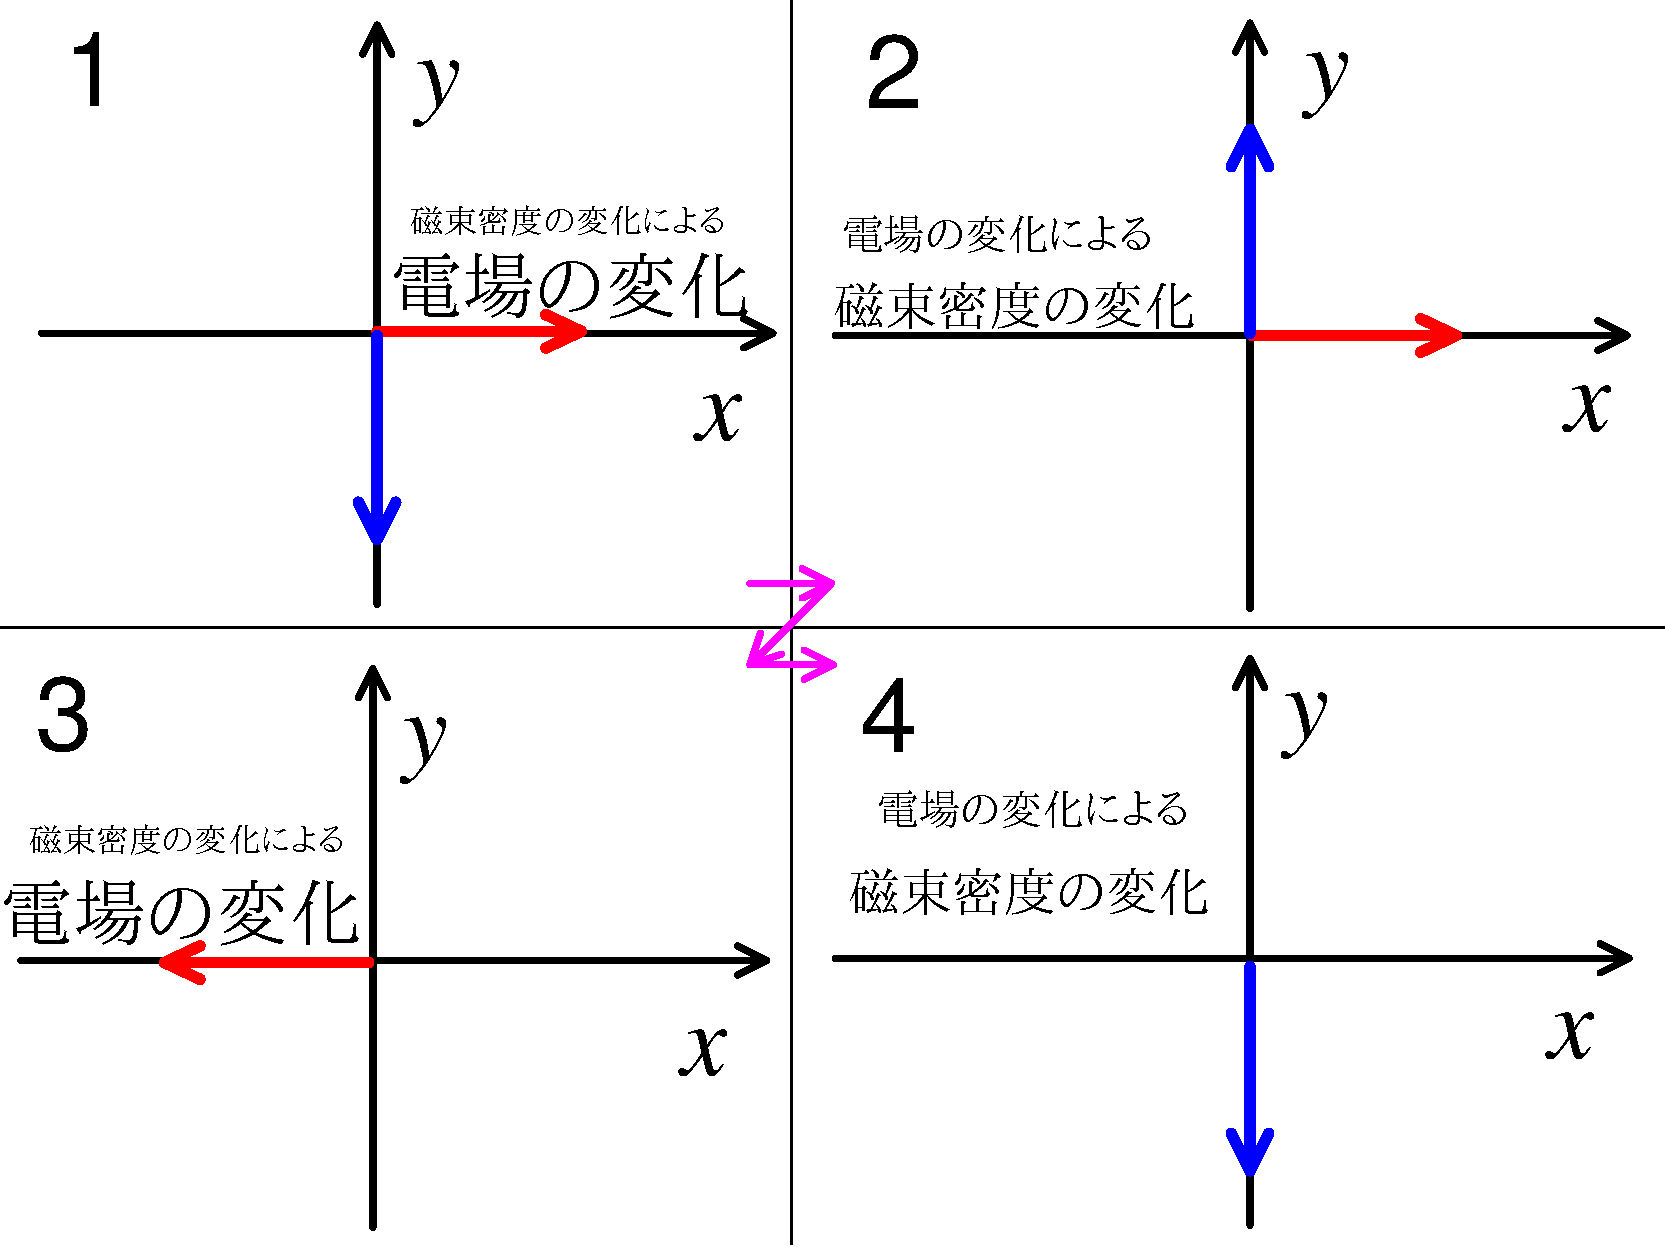
\includegraphics[keepaspectratio, width=6.5cm,height=6cm,clip]{denjiha1.pdf}
                        \caption{原点における電場と磁束密度の変化のイメージ}
                        \label{fig:denjiha1}
                \end{center}
            \end{figure}

            \begin{figure}[hbt]
                \begin{center}
                        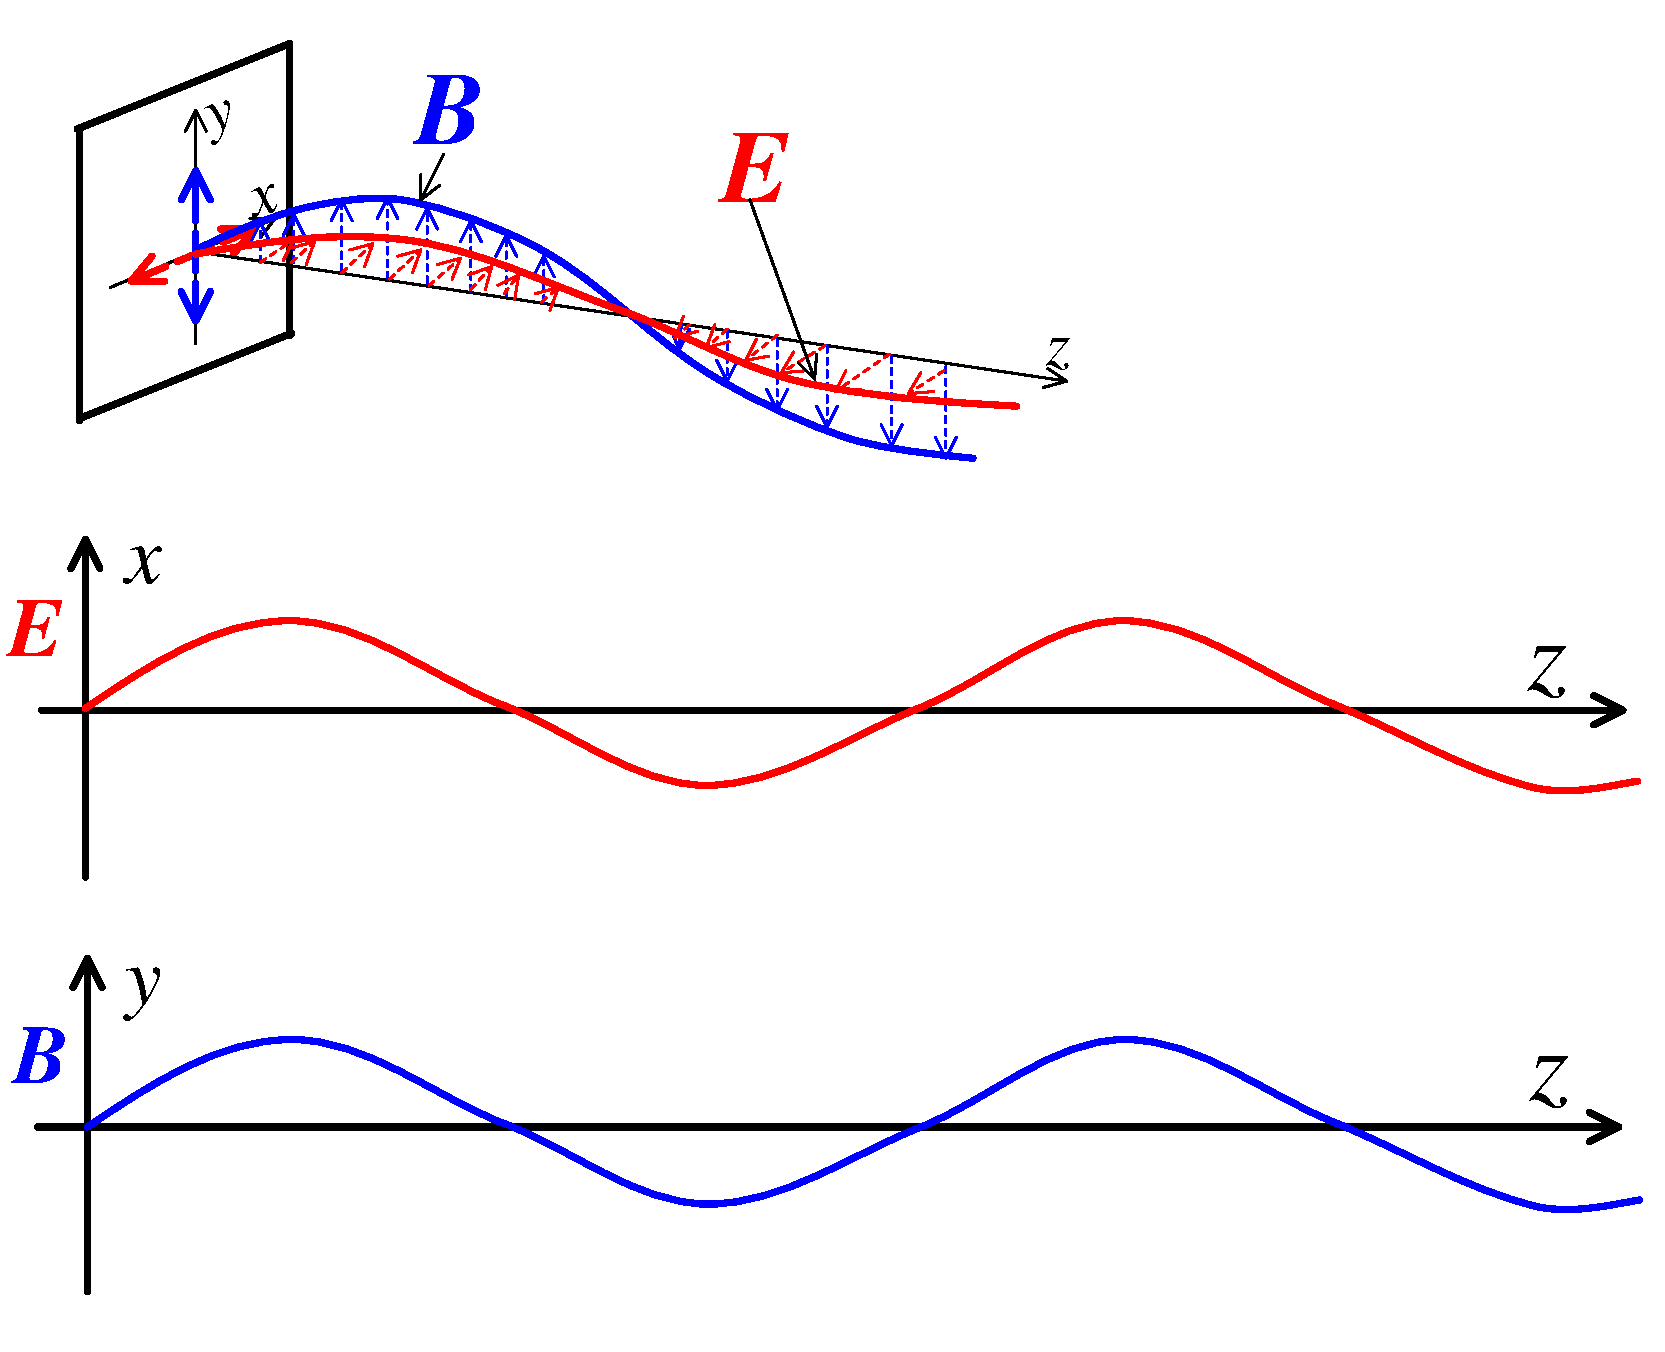
\includegraphics[keepaspectratio, width=6.5cm,height=6cm,clip]{denjiha2.pdf}
                        \caption{電磁波の伝搬のイメージ}
                        \label{fig:denjiha2}
                \end{center}
            \end{figure}

%   %==========================================================================
%   %  SubSection
%   %==========================================================================
    \subsection{電磁場のエネルギー と ポインティング・ベクトル}
        \begin{mycomment}
            電磁波は真空中を伝わる.となると,真空中にも電磁気的なエネルギーが
            蓄えられていると考えられよう.そこで,ここでは真空中に電磁波が存在しているとき,
            この空間に蓄えられている電磁気的なエネルギーについて考える.
        \end{mycomment}

        電磁場におけるエネルギー保存の法則を導く.

        ファラデーの電磁誘導の法則の両辺と,磁束密度 $\bB$ との内積をとり,
                                \begin{align}
                                \bB\cdot\left(\mathrm{rot\,} \bE \right)
                                &= \bB\cdot\left(-\frac{\rd \bB}{\rd t}\right).
                                \end{align}
        右辺を左辺に移項して整理すれば,
                                \begin{align}\label{eq:denyu11}
                                \bB\cdot\left(\frac{\rd \bB}{\rd t}
                                +\mathrm{rot\,} \bE\right)
                                &=0.
                                \end{align}

        次に,アンペール$=$マクスウェルの法則の両辺と,電場 $\bE$ の内積をとり,
                                \begin{align}\label{eq:MAs11}
                                \bE\cdot\mu_{0}\left(\bi+
                                \varepsilon_{0}\frac{\rd \bE}{\rd t}
                                \right)
                                &=\bE\cdot\left(\mathrm{rot\,}
                                \bB\right)
                                \notag \\
                                \Leftrightarrow \quad
                                \bE\cdot\left(
                                \varepsilon_{0}\mu_{0}\frac{\rd \bE}{\rd t}
                                -\mathrm{rot\,}\bB\right)
                                &=-\mu_{0}\bE\cdot\bi
                                \notag \\
                                \Leftrightarrow \quad
                                \bE\cdot\left(
                                \varepsilon_{0}\mu_{0}\frac{\rd \bE}{\rd t}
                                -\mathrm{rot\,}\bB\right)
                                &=-\mu_{0}\bE\cdot\bi
                                \end{align}
        とする.そして,式(\ref{eq:denyu11})と式(\ref{eq:MAs11})の両辺の和をとる.
                                \begin{align}
                                &-\mu_{0}\bE\cdot\bi \notag \\
                                &\quad =
                                \bB\cdot\left(\frac{\rd \bB}{\rd t}
                                +\drot \bE\right)
                                +\bE\cdot\left(
                                \varepsilon_{0}\mu_{0}\frac{\rd \bE}{\rd t}
                                -\drot \bB\right).
                                \end{align}
        右辺と左辺を入れ替えた
                \footnote{
                        A4紙の二段組にした場合,式が一行で納まらなかった.
                }.
            右辺を展開すると,
                                \begin{align}\label{elect_Energy1}
                                &-\mu_{0}\bE\cdot\bi \notag \\
                                &\quad =
                                \bB\cdot\frac{\rd \bB}{\rd t}
                                +\bB\cdot\drot\bE
                                +\bE\cdot\varepsilon_{0}\mu_{0}\frac{\rd \bE}{\rd t}
                                -\bE\cdot\drot\bB.
                                \end{align}

        ところで,任意のベクトル $\bX(t)$ に対して以下の式が成立する.
                                \begin{align}
                                \bX (t)\cdot\frac{\rd \bX (t)}{\rd t}=\frac{1}{2} \frac{\rd \bX(t)^{2}}{ \rd t} .
                                \end{align}
                                \begin{quotation}\small
                                                                なぜなら,
                                \begin{align*}
                                \frac{\rd \bX^{2}}{\rd t}&=\frac{\rd (\bX\cdot \bX)}{\rd t} \\ \notag \\ \notag
                                &=\bX\cdot\frac{\rd  \bX}{\rd t}+\frac{\rd  \bX}{\rd t}\cdot\bX \\ \notag \\ \notag
                                &=2\bX\cdot\frac{\rd \bX}{\rd t}\\ \notag \notag \\
                                \therefore\quad
                                \bX \cdot\frac{\rd \bX }{\rd t}&=\frac{1}{2} \frac{\rd \bX^{2}}{ \rd t} .
                                \end{align*}
                                \end{quotation}

        従って,式(\ref{elect_Energy1})の第1項と第3項を以下のように書き換えることができる.
                                \begin{align*}
                                &-\mu_{0}\bE\cdot\bi \notag \\
                                &\quad = \frac{1}{2} \frac{\rd \bB^{2}}{ \rd t}
                                +\bB\cdot\mathrm{rot\,} \bE
                                +\varepsilon_{0}\mu_{0}\frac{1}{2} \frac{\rd \bE^{2}}{ \rd t}
                                -\bE\cdot\mathrm{rot\,}\bB.
                                \end{align*}
        整理して,
                                \begin{align}
                                &-\mu_{0}\bE\cdot\bi \notag \\
                                &\quad = \frac{1}{2} \frac{\rd }{ \rd t}\left(\bB^{2}
                                +\varepsilon_{0}\mu_{0}\bE^{2}\right)
                                +\bB\cdot\mathrm{rot\,} \bE
                                -\bE\cdot\mathrm{rot\,}\bB.
                                \end{align}
        ここで,左辺の第3項と第4項は,以下のベクトル解析の恒等式を適用してまとめることができる.その公式とは,
        任意の2つのベクトル $\bX$,$\bY$ に対して,
                                \begin{align}
                                \bY\cdot\drot\bX - \bX\cdot\drot\bY =\ddiv(\bX\times\bY).
                                \end{align}
        この恒等式を,上式の左辺第3項と第4項に適用して,式変形すれば,
                                \begin{align}\label{eq:EB_energy}
                                \frac{1}{2} \frac{\rd}{\rd t}\left(\bB^{2}
                                +\varepsilon_{0}\mu_{0}\bE^{2}\right)
                                +\ddiv(\bE\times\bB)
                                =-\mu_{0}\bE\cdot\bi
                                \end{align}
        これを次のように書いてみる.
                                \begin{align}
                                        \ddiv(\bE\times\bB)
                                        + \frac{\rd}{\rd t}
                                          \left\{\frac{1}{2}
                                            \left(
                                              \bB^{2} + \varepsilon_{0}\mu_{0}\bE^{2}
                                            \right)
                                          \right\}
                                        = -\mu_{0}\bE\cdot\bi.
                                \end{align}
        さらに,
                \begin{align}
                        \bS &= \bE\times\bB \,,\,\\
                        W   &= \frac{1}{2} \left(\bB^{2}+\varepsilon_{0}\mu_{0}\bE^{2}\right)
                \end{align}
        と置くと,
            \begin{align}\label{eq:EB_energy}
                \ddiv \bS + \frac{\rd}{\rd t} W = -\mu_{0}\bE\cdot\bi.
            \end{align}
        こうしてみると,式の形が電荷保存の法則の式に似ている.電荷保存の法則は次のように記述された.
            \begin{align}
                 \ddiv\bi + \frac{\rd }{\rd t} \rho = 0.
            \end{align}
        電磁場のエネルギーの式(\ref{eq:EB_energy})の $\bS$ を
        電荷保存の法則の式の電流 $\bi$ と対応させて,
        また,$W$ の部分を電荷密度 $\rho$ と対応させて両式を比較してみよう.

        電荷保存の法則の式の意味は,「電荷の時間変化(つまり電荷の移動)が電流を発生させている」ということであった.
        これを電磁場のエネルギーの式に当てはめて考えると,
        $\left(\bB^{2}+\varepsilon_{0}\mu_{0}\bE^{2}\right)/2$ という
        量の時間変化が,$\ddiv(\bE\times\bB)$ という
        量を生じさせていることになる.また,右辺の電場と電流の積 $-\mu_{0}\bE\cdot\bi$ は
        電荷が電場より受ける単位時間あたりの仕事である.そこで,
        $\left(\bB^{2}+\varepsilon_{0}\mu_{0}\bE^{2}\right)/2$ を \textbf{電磁場のエネルギー密度},
        $\bE\times\bB$ を \textbf{ポインティング・ベクトル} とよぶことにすれば
            \footnote{
                ポインティング・ベクトル:\;Poynting vector であり,ポインティング(Poynting)は
                John Henry Poynting,(1852.9.9-- 1914.3.30,イギリス)
                という人の名前に由来する.
                pointingではない.
            },
        「電磁場のエネルギー密度の変化が,ポインティング・ベクトルを生じさせる」と
        表現される.


